\documentclass{article}

\usepackage{listings}
\usepackage{amsmath}
\usepackage{graphicx}
\usepackage{hyperref}
\usepackage{booktabs}
\usepackage{verbatim}
\usepackage{url}

\begin{document}

\title{Parallel Histogram Calculation in CUDA}
\author{Geoffrey Ulman\\
        CS706}
\date{November 2012}
\maketitle

\section{Glimpse}\label{glimpse}

Glimpse (\url{http://metsci.github.com/glimpse/}) is a Java library for building 2D data visualization applications which take advantage of GPU hardware, allowing users to rapidly explore large data sets\footnote{I have developed Glimpse as part of my professional work over the past year. The development of the graphics library itself is not part of the scope of this project, only the development, profiling, and debugging of the CUDA histogram calculation kernel and the use of Glimpse to visualize the results. Glimpse is released under the open source BSD licence.}. For example, Glimpse uses OpenGL Shader Language (GLSL) to dynamically adjust the color scale of 2D heat map plots like Figure \ref{heatmap}. The underlying data for both the heat map and color scale are stored in OpenGL textures, which allows utilization of the GPU texture cache to speed data lookups.

\begin{figure}
\centering
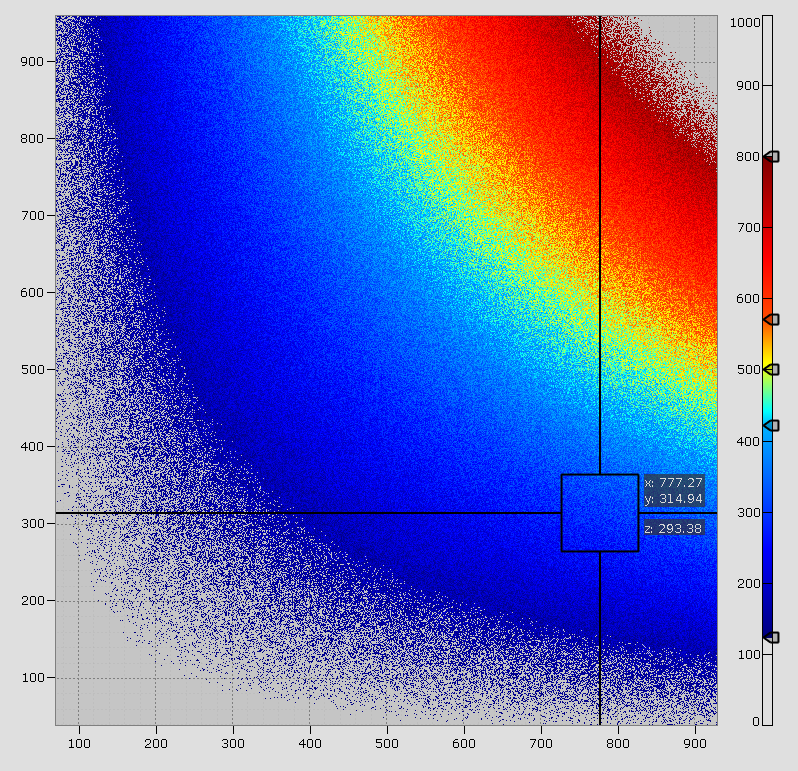
\includegraphics[width=1.0\textwidth]{screenshots/glimpse/TaggedHeatMapExample.png}
\caption{Glimpse Heat Map Visualization\cite{glimpse.com}}
\label{heatmap}
\end{figure}

\section{Abstract}\label{abstract}

While Glimpse supports basic visual effects using OpenGL shaders, more complicated data analysis is better suited for NVIDIA's Compute Unified Device Architecture\cite{cuda-zone} which exposes GPU hardware for general purpose computation. This project uses CUDA to calculate histograms for subsections of a large heat map in real time and displays the results using Glimpse visualization tools. Profiling and optimizing CUDA applications is difficult because computations are run on hudreds of cores simultaneously and multiple interdependent concerns including: register usage, memory access patterns, multiple memory spaces (global, constant, and shared memory), to name only a few, make determining performance bottlenecks difficult. Thus, this project also discusses utilization of NVIDIA's Visual Profiler\cite{nvidia-visual-profiler}.

The input data to the histogram calculation is a matrix of floating point data values. The output is an array of integers containing the number of matrix values which fall within a set of discrete bins. The matrix data is stored in video memory on graphics card as a two dimensional OpenGL texture. This allows the CUDA histogram calculation kernel to take advantage of specialized caching hardware on the graphics card to speed data access.

\begin{figure}
\centering
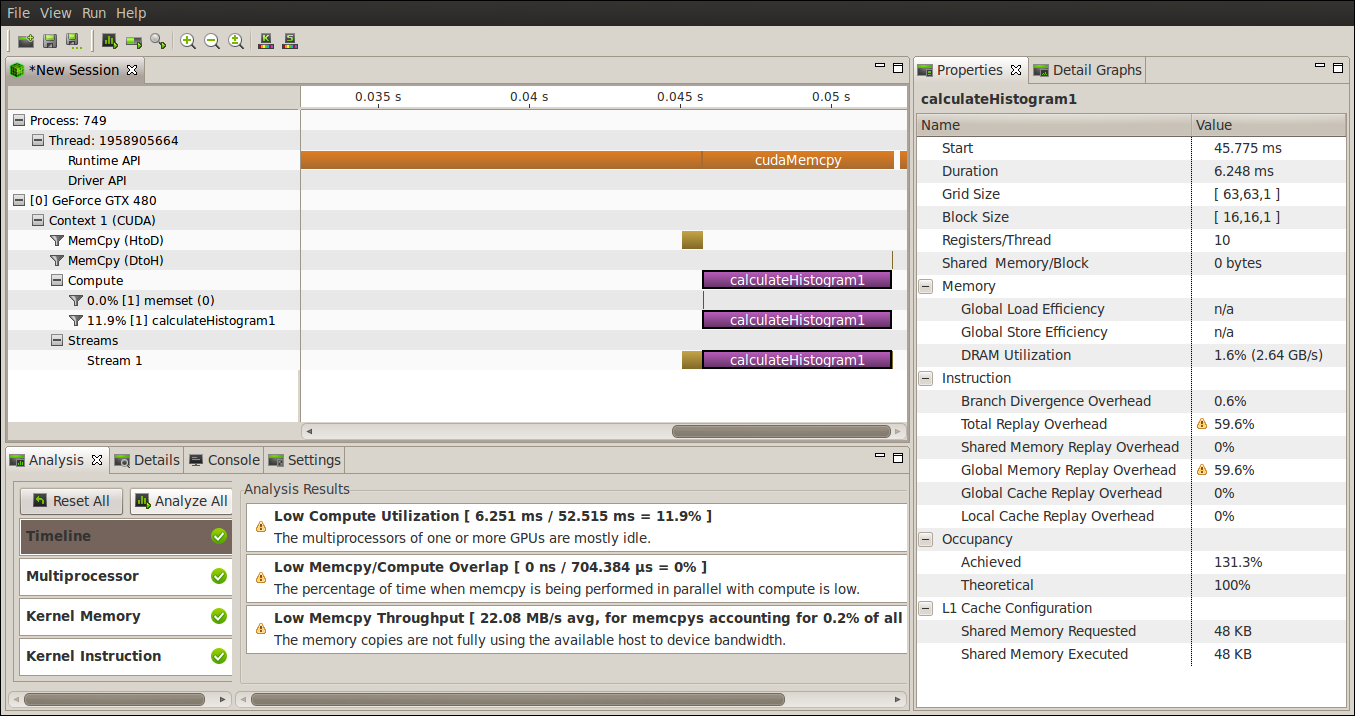
\includegraphics[width=1.0\textwidth]{screenshots/nvvp/calculateHistogram1_screen1.png}
\caption{NVIDIA Visual Profiler running on calculateHistogram1 kernel}
\label{kernel1}
\end{figure}

\section{Approach One}\label{approach1}

CUDA developers write \emph{kernels} which define the behavior of a single logical GPU thread. Threads are grouped into logical \emph{blocks} within which they can share memory and synchronize with one another. They are physically executed on GPU multiprocessors which execute the same instruction on a \emph{warp} of 32 threads simultaneously. Multiprocessor cores have no branch prediction or speculative execution hardware. Instead, they rely on swapping out warps which are blocked on memory access or slow operations to keep the multiprocessor busy. 

Because of this Single Instruction, Multiple Thread (SIMT) data parallel programming model, often the first question which must be asked when designing a CUDA algorithm is how GPU threads will map to data. For the histogram calculation problem, the simplest approach is to simply assign one thread to each matrix/texture element. That thread will determine the appropriate bin for its data value, and increment the bin by one.

\lstset{language=C,basicstyle=\footnotesize}
\begin{minipage}{\textwidth}
\begin{lstlisting}[caption=Global Memory atomicAdd kernel]
__global__ void calculateHistogram1( int *bins, int nbins,
                                     float minX, float stepX,
                                     float minY, float stepY,
                                     float minZ, float maxZ )
{
    // use block and thread ids to get texture coordinates for this thread
    int i = blockIdx.x * blockDim.x + threadIdx.x;
    int j = blockIdx.y * blockDim.y + threadIdx.y;

    // convert block/thread ids into texture coordinates
    float x = minX + stepX * i;
    float y = minY + stepY * j;

    // don't over count if texture coordinates are out of bounds
    if ( x < 1.0 && y < 1.0 )
    {
        // perform texture lookup
        float result = tex2D(texture_float_2D, x, y);
    
        // calculate bin index
        float stepZ = ( maxZ - minZ ) / nbins;
        float fbinIndex = floor( ( result - minZ ) / stepZ );
        int binIndex = (int) clamp( fbinIndex, 0, nbins-1 );
    
        // atomically add one to the bin corresponding to the data value
        atomicAdd( bins+binIndex, 1 );
    }
}
\end{lstlisting}
\end{minipage}

\bibliographystyle{plain}
\bibliography{report}

\end{document}
